\documentclass[12pt,a4paper]{article}

\usepackage[T1]{fontenc}
\usepackage[utf8]{inputenc}
\usepackage{mathptmx}
\renewcommand{\sfdefault}{ptm}
\usepackage{microtype}
\usepackage{amsmath}
\usepackage{textcomp}
\usepackage[a4paper,margin=2.5cm,headheight=14pt]{geometry}
\usepackage{xcolor}
\usepackage{booktabs,tabularx,threeparttable}
\newcolumntype{Y}{>{\raggedright\arraybackslash}X}
\usepackage{enumitem}
\usepackage{caption}
\usepackage{titlesec}
\usepackage{needspace}
\usepackage{fancyhdr}
\usepackage[round,authoryear]{natbib}
\usepackage{pgfplots}
\pgfplotsset{compat=1.18,
  xticklabel={\pgfmathprintnumber[assume math mode=true]{\tick}},
  yticklabel={\pgfmathprintnumber[assume math mode=true]{\tick}}}
\usetikzlibrary{positioning,arrows.meta,shapes.geometric}
\usepackage[hidelinks]{hyperref}
\urlstyle{same}

\definecolor{ink}{HTML}{1D1C1A}
\definecolor{quiet}{HTML}{6B675F}
\definecolor{rule}{HTML}{D9D4C7}
\definecolor{accent}{HTML}{2F5D8A}
\definecolor{grey}{HTML}{B9B4A9}
\definecolor{red}{HTML}{B42A2A}
\definecolor{gold}{HTML}{B8860B}
\definecolor{boxbg}{HTML}{F1EEE6}

\hypersetup{colorlinks=true,linkcolor=accent,citecolor=accent,urlcolor=accent}

\titleformat{\section}{\needspace{7\baselineskip}\sffamily\large\bfseries\color{ink}}{\thesection}{0.8em}{}
\titleformat{\subsection}{\needspace{6\baselineskip}\sffamily\normalsize\bfseries\color{ink}}{\thesubsection}{0.8em}{}
\titlespacing*{\section}{0pt}{1.6em}{0.6em}
\titlespacing*{\subsection}{0pt}{1.1em}{0.4em}
\captionsetup{font={small,sf},labelfont=bf,labelsep=period,justification=raggedright,singlelinecheck=false}
\setlist{itemsep=0.25em,topsep=0.4em}
\setlength{\parskip}{0.45em}
\setlength{\parindent}{0pt}

\pagestyle{fancy}
\fancyhf{}
\fancyhead[L]{\sffamily\footnotesize\color{quiet}Case study: Esports Intelligence}
\fancyhead[R]{\sffamily\footnotesize\color{quiet}Nahian Ibnat}
\fancyfoot[C]{\sffamily\footnotesize\color{quiet}\thepage}
\renewcommand{\headrulewidth}{0.4pt}
\renewcommand{\headrule}{\hbox to\headwidth{\color{rule}\leaders\hrule height \headrulewidth\hfill}}

\newcommand{\keybox}[2]{%
  \par\noindent\colorbox{boxbg}{\parbox{\dimexpr\linewidth-2\fboxsep}{\vspace{0.3em}%
  {\sffamily\small\bfseries\color{accent}#1}\par\vspace{0.2em}\small #2\vspace{0.3em}}}\par}

\begin{document}

\thispagestyle{empty}
{\sffamily\small\color{red}\textbf{CASE STUDY} \textbar{} SPORTS ANALYTICS AND FORECASTING}\par
\vspace{0.6em}
{\LARGE\bfseries\color{ink} Does Machine Learning Beat Elo?\par}
\vspace{0.3em}
{\Large\color{quiet} Rating design, model choice and player information in professional League of Legends\par}
\vspace{1em}
{\sffamily\normalsize\textbf{Nahian Ibnat}}\par
{\sffamily\small\color{quiet} Independent research project \textbar{} November 2026}\par
\vspace{0.8em}
{\color{rule}\rule{\linewidth}{0.6pt}}

\keybox{Executive summary}{%
This case study documents the design, evaluation and deployment of \emph{Esports Intelligence}, a public research platform built on 75,830 professional League of Legends games from January 2020 to November 2026. The project asked whether machine learning predicts the winner of a game better than an Elo rating. On 10,087 games it had never seen, a logistic regression beat calibrated Elo by 0.0006 in Brier score (0.2164 against 0.2170): a gain that is statistically real but about 0.3\% of the score. Two simpler changes mattered far more. Giving each league its own rating level improved Elo by 0.0054, and adding one measure of player experience, known before match day, improved the logistic model by 0.0048. Both effects held in each of five separate test years (2022 to 2026, 49,748 games), and the player effect was the same size inside single leagues, so it is not a proxy for league strength. The lesson is that what a rating knows matters more than which model uses it.}

\vspace{0.5em}
{\small\textbf{Keywords:} forecasting, Elo rating, logistic regression, Brier score, esports, time-ordered evaluation, cluster bootstrap}

\section{Background}

Elo ratings are the standard way to predict who wins a game. Each competitor has a number; the gap between two numbers gives a win probability, and after each game the winner takes points from the loser, more so when the result is a surprise \citep{elo1978}. The system was designed for chess \citep{elo1978}; FIFA's men's world ranking has used an Elo-based method since August 2018 \citep{fifa2018}; and the official power rankings of professional League of Legends are built on Elo \citep{riot2024}. Elo ratings also have a long record as predictors of match results \citep{hvattum2010}.

Machine learning models can use far more information than a single rating. The practical question for any forecaster is whether that extra information pays for the extra complexity, and by how much. Professional League of Legends is a useful setting for this question for three reasons:

\begin{itemize}
  \item \textbf{Data.} Every professional game is recorded in detail and published, with one row per team and one per player \citep{oracleselixir}.
  \item \textbf{Volume.} Teams play often: the files used here hold 75,830 games from January 2020 to November 2026 \citep{oracleselixir,ei2026}.
  \item \textbf{Structure.} The data covers 109 leagues \citep{ei2026}. Teams play most of their games inside their own league (39,185 of the 49,748 five-year test games, 79\%, were domestic games between teams of the same league; \citealp{ei2026}), and leagues meet mainly at international events such as MSI and Worlds, which is why Riot's own rankings let those events set each league's strength \citep{riot2024}. Comparing teams that rarely play each other is therefore a real measurement problem.
\end{itemize}

\section{The problem}

\keybox{Central research question}{Can machine learning predict the winner of a professional League of Legends game, before it starts, better than an Elo rating?}

As the work progressed, four further questions followed from the results:
\begin{enumerate}[label=\textbf{Q\arabic*.},leftmargin=2.4em]
  \item How much does the design of the rating itself matter, compared with the choice of model?
  \item Do the results hold beyond a single test period?
  \item Does information about the players add what team ratings miss?
  \item If it does, is the player effect simply a sign of league strength?
\end{enumerate}

A second aim was practical: to make every step public and checkable, as a live website, rather than report a single accuracy number.

\section{Data}

All data comes from the public historical files of Oracle's Elixir \citep{oracleselixir}. The study uses every file from 2020 to November 2026: 75,830 games, 1,914 teams and 10,239 players across 109 leagues, played between 3 January 2020 and 17 November 2026 (counts from the project database; \citealp{ei2026}). Each raw file is recorded in a manifest with its SHA-256 checksum, so the exact input can be verified.

The data was usable but not clean enough to trust as delivered. Table~\ref{tab:data} lists the problems found and how each was handled. Every exclusion is written to a file with its reason and shown in the platform's public data quality report.

\begin{table}[h]
\centering\small
\caption{Data problems and how they were handled}\label{tab:data}
\begin{tabularx}{\linewidth}{@{}>{\raggedright\arraybackslash}p{4.6cm}Y@{}}
\toprule
Problem & Treatment \\
\midrule
Duplicate and conflicting rows & Exact duplicates dropped (one kept); conflicting rows for the same game and player dropped entirely and reported \\
Games without exactly two teams, one blue and one red, and one winner & Excluded, with the reason recorded \\
Missing statistics & Kept as missing, never filled with zero; averages use only games where the value exists \\
No series identifier in the source & Best-of-three and best-of-five series rebuilt from game times and the source's game number \\
Season label differs from calendar year & Some late-2026 qualifiers are labelled 2027; ratings use the game date, season tables use the label \\
\bottomrule
\end{tabularx}
\end{table}

\section{Approach}

\subsection{Prediction task and evaluation design}

The task is to predict, before a game starts, the probability that the blue side wins. The design follows how a forecaster would actually be used:

\begin{enumerate}
  \item \textbf{Split by date, never at random.} Models are trained on games up to 11 August 2024, tuned on games up to 22 September 2025, and scored once on 10,087 games from 23 September 2025 to 14 November 2026. A random split would let a model learn from the future.
  \item \textbf{Use only earlier information.} Every input to a prediction comes from games played strictly before it. Automated tests change future results and lineups and check that earlier inputs do not move.
  \item \textbf{Compare against simple baselines.} A constant blue-side win rate, Elo, and calibrated Elo. A model is useful only if it beats these clearly.
  \item \textbf{Score probabilities, not only picks.} The main measure is the Brier score \citep{brier1950}, the mean squared gap between the predicted probability and the result; lower is better and a constant 50\% scores 0.25. Log loss, accuracy and ROC-AUC \citep{fawcett2006} are also reported.
  \item \textbf{Put an interval on every difference.} Model differences use a paired bootstrap \citep{efron1979} with 2,000 resamples. Games from the same series are resampled together, because they are not independent \citep{cameron2008}; the check is repeated with whole tournaments as the unit.
  \item \textbf{Keep statistical and practical size apart.} A difference can be real and still too small to matter.
\end{enumerate}

\subsection{Models}

Table~\ref{tab:models} summarises the models. Elo settings and the regression penalty were chosen on the validation period only. The regressions use scikit-learn \citep{pedregosa2011}. Gradient boosting \citep{friedman2001} and random forests \citep{breiman2001} were also tested; they did not beat the logistic regression on validation games and were not used.

\begin{table}[h]
\centering\small
\caption{Models compared}\label{tab:models}
\begin{tabularx}{\linewidth}{@{}>{\raggedright\arraybackslash}p{4.3cm}Y@{}}
\toprule
Model & Inputs \\
\midrule
Constant baseline & Blue-side win rate of earlier games \\
Elo with league levels & Team rating = league level + team component; league levels move only in games between leagues (K\,=\,40) \\
Calibrated Elo & Logistic regression on the Elo difference; the intercept estimates the blue-side advantage \\
Logistic regression & Six pre-game features: Elo difference, recent form, overall win rate, strength of recent opponents, experience, and an international-event term \\
Logistic + player experience & The six features plus the difference in mean log(1\,+\,earlier professional games) of each team's players in its previous game \\
\bottomrule
\end{tabularx}
\end{table}

\subsection{Robustness checks}

After the first results, three checks were added:
\begin{itemize}
  \item \textbf{Five-year rolling test.} For each test year \textit{Y} from 2022 to 2026, models are trained on years before \textit{Y}\,\textminus\,1, tuned on \textit{Y}\,\textminus\,1 and scored on \textit{Y}, with every model re-tuned each year.
  \item \textbf{Player features.} The source lists the five players in every game. Features were built from each team's previous lineup (known before match day) and, for comparison, from the lineup that played (known only when the game starts).
  \item \textbf{Subgroups.} Test games were split by type, including games between two teams of the same league, where league levels cancel out.
\end{itemize}

\section{Implementation}

The research was built as a public website so that others can check it (Figure~\ref{fig:arch}). A data pipeline validates and loads the files into PostgreSQL; a training step fits the models and writes model versions and predictions to the database; a FastAPI service serves ratings, predictions and statistics; and a Next.js site presents them, including a prediction lab and an experiments page. All hosting uses free tiers (Supabase, Render, Vercel). Because the free API server sleeps when unused, common views are served from a saved snapshot, and a monitor pings a health check every five minutes. The code has 105 backend tests, including database integration tests and a test that the live API computes exactly the same player feature the model was trained on.

\begin{figure}[h]
\centering
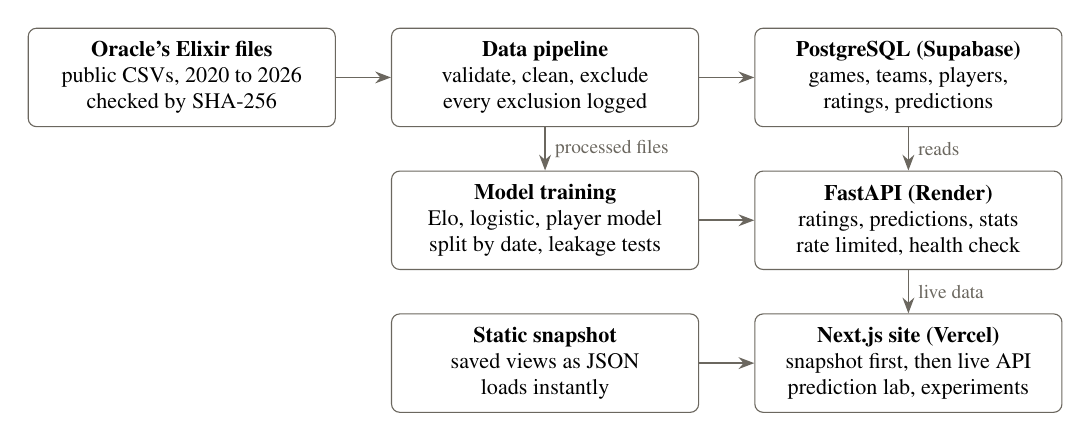
\begin{tikzpicture}[
  node distance=0.55cm and 0.7cm,
  every node/.style={font=\sffamily\footnotesize},
  box/.style={draw=quiet,rounded corners=3pt,align=center,minimum width=3.9cm,minimum height=1.25cm,fill=white},
  arr/.style={-{Stealth[length=2mm]},draw=quiet,line width=0.6pt},
  lab/.style={font=\sffamily\scriptsize,text=quiet}]
\node[box] (src) {\textbf{Oracle's Elixir files}\\public CSVs, 2020 to 2026\\checked by SHA-256};
\node[box,right=of src] (pipe) {\textbf{Data pipeline}\\validate, clean, exclude\\every exclusion logged};
\node[box,right=of pipe] (db) {\textbf{PostgreSQL (Supabase)}\\games, teams, players,\\ratings, predictions};
\node[box,below=of pipe] (train) {\textbf{Model training}\\Elo, logistic, player model\\split by date, leakage tests};
\node[box,below=of db] (api) {\textbf{FastAPI (Render)}\\ratings, predictions, stats\\rate limited, health check};
\node[box,below=of train] (snap) {\textbf{Static snapshot}\\saved views as JSON\\loads instantly};
\node[box,below=of api] (site) {\textbf{Next.js site (Vercel)}\\snapshot first, then live API\\prediction lab, experiments};
\draw[arr] (src) -- (pipe);
\draw[arr] (pipe) -- (db);
\draw[arr] (pipe) -- node[lab,right]{processed files} (train);
\draw[arr] (train) -- (api);
\draw[arr] (db) -- node[lab,right]{reads} (api);
\draw[arr] (api) -- node[lab,right]{live data} (site);
\draw[arr] (snap) -- (site);
\end{tikzpicture}
\caption{System architecture. Training also writes model versions and test predictions to the database.}\label{fig:arch}
\end{figure}

\section{Results}

All results in this section come from the project's saved evaluation files and experiment record \citep{ei2026}.

\subsection{Machine learning wins, but only just}

Table~\ref{tab:main} shows the main test results. The logistic regression beats calibrated Elo by 0.00062 in Brier score, with a 95\% interval of 0.00023 to 0.00104; the interval also excludes zero when whole tournaments are resampled. The gain is real, but it is about 0.3\% of the score, and both models pick the right winner about 65\% of the time.

\begin{table}[h]
\centering\small
\begin{threeparttable}
\caption{Main test results (10,087 games, 23 September 2025 to 14 November 2026)}\label{tab:main}
\begin{tabular}{@{}lcccc@{}}
\toprule
Model & Brier & Log loss & Accuracy & ROC-AUC \\
\midrule
Constant blue-side rate & 0.2488 & 0.6908 & 53.5\% & n/a \\
Elo with league levels & 0.2176 & 0.6249 & 64.7\% & 0.705 \\
Calibrated Elo & 0.2170 & 0.6232 & 64.8\% & 0.705 \\
Logistic regression & 0.2164 & 0.6215 & 64.9\% & 0.707 \\
\textbf{Logistic + player experience} & \textbf{0.2116} & \textbf{0.6104} & \textbf{65.7\%} & \textbf{0.721} \\
\bottomrule
\end{tabular}
\begin{tablenotes}\footnotesize
\item Lower is better for Brier score and log loss. All models are scored on the same games.
\end{tablenotes}
\end{threeparttable}
\end{table}

\subsection{The rating design matters more than the model}

The first Elo version put every team on one scale. It ranked teams from small regional leagues above the best teams in Korea and China, because they beat their neighbours and rarely played anyone else. Since Elo points move between leagues only when their teams meet, a single scale cannot be right. Giving each league its own level, learned only from games between leagues, lowered the Brier score by 0.0054 (95\% interval 0.0041 to 0.0068), about nine times the machine learning gain. The design follows the same idea as the industry's own ratings, which blend a team Elo with a league Elo \citep{riot2024}.

\subsection{Player experience helps most}

Adding one number, the average earlier professional games of the players in each team's previous game, lowered the Brier score by 0.0048 (95\% interval 0.0035 to 0.0060), about eight times the machine learning gain. Figure~\ref{fig:gains} compares the three steps on the same games.

\begin{figure}[h]
\centering
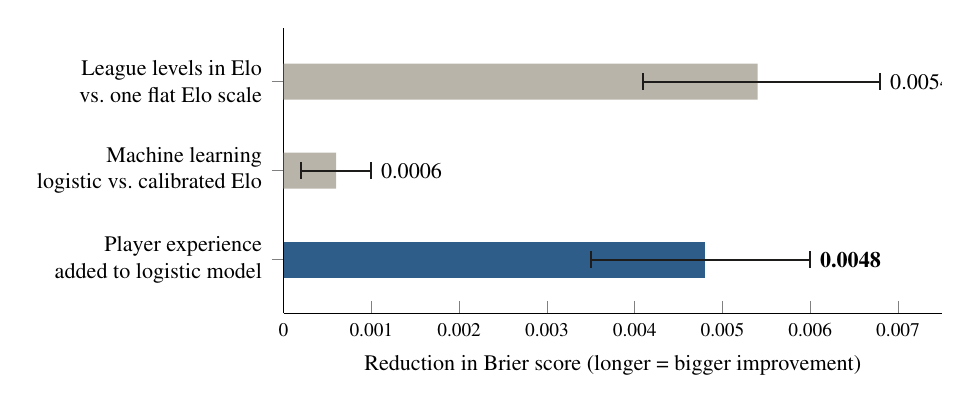
\begin{tikzpicture}
\begin{axis}[
  xbar, width=0.82\linewidth, height=5.2cm,
  xmin=0, xmax=0.0075, bar width=13pt, bar shift=0pt,
  ytick={1,2,3},
  yticklabels={{Player experience\\added to logistic model},{Machine learning\\logistic vs.\ calibrated Elo},{League levels in Elo\\vs.\ one flat Elo scale}},
  yticklabel style={align=right,font=\sffamily\footnotesize},
  xticklabel style={font=\sffamily\scriptsize,/pgf/number format/fixed,/pgf/number format/precision=3},
  scaled x ticks=false,
  xlabel={\sffamily\footnotesize Reduction in Brier score (longer = bigger improvement)},
  axis x line*=bottom, axis y line*=left,
  enlarge y limits=0.3,
  error bars/x dir=both, error bars/x explicit,
  error bars/error bar style={line width=0.7pt,ink},
  error bars/error mark options={rotate=90,mark size=3pt,line width=0.7pt,ink},
]
\addplot[fill=grey,draw=none] coordinates {
  (0.0054,3) += (0.0014,0) -= (0.0013,0)
  (0.0006,2) += (0.0004,0) -= (0.0004,0)
};
\addplot[fill=accent,draw=none] coordinates {
  (0.0048,1) += (0.0012,0) -= (0.0013,0)
};
\node[right,font=\sffamily\footnotesize] at (axis cs:0.0068,3) {0.0054};
\node[right,font=\sffamily\footnotesize] at (axis cs:0.0010,2) {0.0006};
\node[right,font=\sffamily\footnotesize\bfseries] at (axis cs:0.0060,1) {0.0048};
\end{axis}
\end{tikzpicture}
\caption{Improvement from each step on the same 10,087 test games. Error bars show 95\% intervals from a series-clustered bootstrap.}\label{fig:gains}
\end{figure}

\subsection{The results hold in every year}

In the five-year rolling test, league levels improved Elo in all five years and player experience improved the logistic model in all five years, while the machine learning step stayed close to zero: 0.0004 pooled over 49,748 games, with an interval excluding zero in only two of the five years (Figure~\ref{fig:years}).

\begin{figure}[h]
\centering
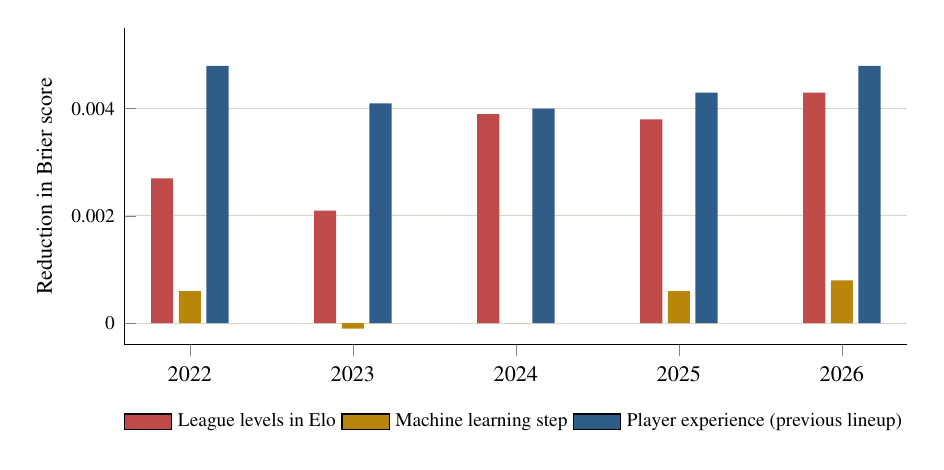
\begin{tikzpicture}
\begin{axis}[
  ybar, width=0.95\linewidth, height=5.6cm,
  bar width=8pt, ymin=-0.0004, ymax=0.0055,
  symbolic x coords={2022,2023,2024,2025,2026}, xtick=data,
  xticklabel style={font=\sffamily\footnotesize},
  yticklabel style={font=\sffamily\scriptsize,/pgf/number format/fixed,/pgf/number format/precision=3},
  scaled y ticks=false,
  ylabel={\sffamily\footnotesize Reduction in Brier score},
  axis x line*=bottom, axis y line*=left,
  legend style={font=\sffamily\scriptsize,draw=none,at={(0.5,-0.18)},anchor=north,legend columns=3},
  legend cell align=left, area legend,
  ymajorgrids, grid style={rule},
]
\addplot[fill=red!85,draw=none] coordinates {(2022,0.0027) (2023,0.0021) (2024,0.0039) (2025,0.0038) (2026,0.0043)};
\addplot[fill=gold,draw=none] coordinates {(2022,0.0006) (2023,-0.0001) (2024,0.0000) (2025,0.0006) (2026,0.0008)};
\addplot[fill=accent,draw=none] coordinates {(2022,0.0048) (2023,0.0041) (2024,0.0040) (2025,0.0043) (2026,0.0048)};
\legend{League levels in Elo, Machine learning step, Player experience (previous lineup)}
\end{axis}
\end{tikzpicture}
\caption{The same three steps by test year. Each year the models were tuned and fitted only on earlier years.}\label{fig:years}
\end{figure}

Table~\ref{tab:ablation} shows which part of player information matters. One simple number does most of the work; knowing the lineup that actually played helps a little more, but most of the gain is already there before match day.

\begin{table}[h]
\centering\small
\begin{threeparttable}
\caption{Player features added to the logistic model, five-year test (49,748 games)}\label{tab:ablation}
\begin{tabular}{@{}lcc@{}}
\toprule
Added feature & Brier change & Better in \\
\midrule
Lineup continuity (same players as last game) & \textminus0.0001 & 4 of 5 years \\
Player tenure with the team & \textminus0.0007 & 5 of 5 \\
Player experience, previous lineup (pre-match) & \textminus0.0044 & 5 of 5 \\
Player experience, lineup that played & \textminus0.0055 & 5 of 5 \\
Pre-match experience + player-level Elo & \textminus0.0053 & 5 of 5 \\
\bottomrule
\end{tabular}
\begin{tablenotes}\footnotesize
\item Negative values mean better predictions. Pooled over all test years.
\end{tablenotes}
\end{threeparttable}
\end{table}

\subsection{It is not just league strength}

If experienced players are concentrated in strong leagues, the player measure could simply be separating strong leagues from weak ones. In a game between two teams of the same league the league level cancels out, so league strength cannot explain a gain there. Table~\ref{tab:sub} shows that the gain is the same size inside a single league, and largest for new teams, which Elo rates at their league's average even when their players have hundreds of games behind them.

\begin{table}[h]
\centering\small
\begin{threeparttable}
\caption{Pre-match player model against the logistic model, by type of game}\label{tab:sub}
\begin{tabular}{@{}lrc@{}}
\toprule
Games & \textit{n} & Brier change [95\% interval] \\
\midrule
Same league, domestic game & 39,185 & \textminus0.0053 [\textminus0.0060, \textminus0.0047] \\
Top leagues only (LCK, LPL, LEC, LCS / LTA North) & 8,600 & \textminus0.0027 [\textminus0.0037, \textminus0.0016] \\
Teams from different leagues & 10,229 & \textminus0.0052 [\textminus0.0064, \textminus0.0039] \\
Both teams with 20 or more earlier games & 42,314 & \textminus0.0043 [\textminus0.0049, \textminus0.0037] \\
A team with fewer than 20 earlier games & 7,434 & \textminus0.0108 [\textminus0.0129, \textminus0.0089] \\
\bottomrule
\end{tabular}
\begin{tablenotes}\footnotesize
\item Five-year test games. Negative values mean better predictions.
\end{tablenotes}
\end{threeparttable}
\end{table}

\section{Discussion and lessons}

\textbf{What the model knows beats what kind of model it is.} League structure and player experience moved the score far more than switching from a rating to machine learning. The type of model mattered little once the rating measured the right things.

\textbf{A real result can be a small one.} The machine learning gain passed every significance check and still did not matter much in practice. Reporting both is the honest answer, and it is the kind of distinction that a single accuracy figure hides.

\textbf{Check your own headline.} The first published conclusion was correct but incomplete. The five-year test and the player features found a larger effect that the original design had left out.

\textbf{Data rules are research decisions.} How series are rebuilt, what counts as a duplicate and what is excluded all change the numbers, so they are written down and made public.

\textbf{Relation to earlier work.} The results agree with work showing that player-based ratings improve football forecasts \citep{holmes2024} and that player-level performance measures improve League of Legends ratings \citep{debois2025}. Earlier studies of professional League games report accuracy on a single sample \citep{jadowski2022}. This study adds a paired, time-ordered comparison of rating design, model type and player information on the same games, checked over five years and inside single leagues.

\section{Limitations}

\begin{itemize}
  \item Player experience is associated with winning, but this does not show that it causes wins: it may reflect skill, or which players strong organisations choose to sign.
  \item The pre-match model uses each team's previous lineup, so it does not see a lineup change made since the last game.
  \item League levels are only well measured for leagues that often play other leagues.
  \item Series are rebuilt from game times, because the source has no series identifier.
  \item No draft, patch or in-game information is used, and the models are fixed at the start of each test period.
\end{itemize}

\section{Recommendations and next steps}

\begin{enumerate}
  \item \textbf{Compare with established rating systems} such as Glicko-2 \citep{glickman2001} and TrueSkill \citep{herbrich2007}, which model rating uncertainty and may help with new teams.
  \item \textbf{Test other definitions of experience}, such as recent games only or top-league games only, to check that the result does not depend on one definition.
  \item \textbf{Compare with betting odds.} If bookmaker odds already reflect player experience, the gain is public information that markets price in; if not, the result says something about market efficiency.
\end{enumerate}

\section*{Resources}
\begin{itemize}[leftmargin=1.2em]
  \item Live platform: \url{https://esports-intelligence.vercel.app}
  \item Five-year results: \url{https://esports-intelligence.vercel.app/experiments}
  \item Research article: \url{https://nahianibnat-2000.github.io/esports-intelligence/}
  \item Code, tests and experiment records:\\ \url{https://github.com/NahianIbnat-2000/esports-intelligence}
\end{itemize}

\begin{thebibliography}{99}
\setlength{\itemsep}{0.2em}\small
\bibitem[Breiman(2001)]{breiman2001} Breiman, L. (2001). Random forests. \emph{Machine Learning}, 45(1), 5--32.
\bibitem[Cameron et~al.(2008)]{cameron2008} Cameron, A.~C., Gelbach, J.~B., and Miller, D.~L. (2008). Bootstrap-based improvements for inference with clustered errors. \emph{Review of Economics and Statistics}, 90(3), 414--427.
\bibitem[Brier(1950)]{brier1950} Brier, G.~W. (1950). Verification of forecasts expressed in terms of probability. \emph{Monthly Weather Review}, 78(1), 1--3.
\bibitem[De Bois et al.(2025)]{debois2025} De Bois, M., Parmentier, F., Puget, R., Tanti, M., and Peltier, J. (2025). PandaSkill: player performance and skill rating in esports, application to League of Legends. arXiv:2501.10049.
\bibitem[Efron(1979)]{efron1979} Efron, B. (1979). Bootstrap methods: another look at the jackknife. \emph{Annals of Statistics}, 7(1), 1--26.
\bibitem[Elo(1978)]{elo1978} Elo, A.~E. (1978). \emph{The Rating of Chessplayers, Past and Present}. New York: Arco.
\bibitem[Fawcett(2006)]{fawcett2006} Fawcett, T. (2006). An introduction to ROC analysis. \emph{Pattern Recognition Letters}, 27(8), 861--874.
\bibitem[FIFA(2018)]{fifa2018} FIFA (2018). FIFA/Coca-Cola Men's World Ranking: procedures. \url{https://inside.fifa.com/fifa-world-ranking/procedure-men}
\bibitem[Friedman(2001)]{friedman2001} Friedman, J.~H. (2001). Greedy function approximation: a gradient boosting machine. \emph{Annals of Statistics}, 29(5), 1189--1232.
\bibitem[Glickman(2001)]{glickman2001} Glickman, M.~E. (2001). Dynamic paired comparison models with stochastic variances. \emph{Journal of Applied Statistics}, 28(6), 673--689.
\bibitem[Herbrich et~al.(2007)]{herbrich2007} Herbrich, R., Minka, T., and Graepel, T. (2007). TrueSkill: a Bayesian skill rating system. In \emph{Advances in Neural Information Processing Systems 19}, 569--576.
\bibitem[Holmes and McHale(2024)]{holmes2024} Holmes, B. and McHale, I.~G. (2024). Forecasting football match results using a player rating based model. \emph{International Journal of Forecasting}, 40(1), 302--312.
\bibitem[Hvattum and Arntzen(2010)]{hvattum2010} Hvattum, L.~M. and Arntzen, H. (2010). Using ELO ratings for match result prediction in association football. \emph{International Journal of Forecasting}, 26(3), 460--470.
\bibitem[Ibnat(2026)]{ei2026} Ibnat, N. (2026). Esports Intelligence: data pipeline, code, evaluation files and experiment records. GitHub repository. \url{https://github.com/NahianIbnat-2000/esports-intelligence}
\bibitem[Jadowski and Cunningham(2022)]{jadowski2022} Jadowski, R. and Cunningham, S. (2022). Statistical models for predicting results in professional League of Legends. In \emph{ArtsIT, Interactivity and Game Creation: Creative Heritage}.
\bibitem[Pedregosa et~al.(2011)]{pedregosa2011} Pedregosa, F. et~al. (2011). Scikit-learn: machine learning in Python. \emph{Journal of Machine Learning Research}, 12, 2825--2830.
\bibitem[Riot Games(2024)]{riot2024} Riot Games (2024). Dev diary: unveiling the Global Power Rankings. LoL Esports. \url{https://lolesports.com/en-GB/news/dev-diary-unveiling-the-global-power-rankings}
\bibitem[Sevenhuysen(2026)]{oracleselixir} Sevenhuysen, T. (2026). Oracle's Elixir: League of Legends esports match data. \url{https://oracleselixir.com}
\end{thebibliography}

\end{document}
